PLATO (PLanetary Transits and Oscillations of stars) is an ESA mission launching in late 2024 with the goal of finding terrestrial exoplanets within the habitable zone of solar-like stars. The mission will be delivered with a Soyuz 2-1b launch vehicle with Fregat-MT upper stage. The satellite will be placed in a large amplitude liberation orbit around the earth-sun lagrange point 2 (L2 Point). In its orbit it will conduct multiple ultra-high precision, long duration, uninterrupted photometric monitoring of at least two different star fields over two years each. After that, a "step-and-stare" phase will be started, in which the spacecraft is pointed to areas of special interest for several months. This phase will last for another two years. Two additional years of use of the satellite are possible. To guarantee a continuous power supply, the spacecraft has to be rotated around its line of sight every three months to make sure its solar arrays are pointed to the sun. This has to happen without altering the line of sight between spacecraft and the observed sky array.
\newline
In this chapter the specifications and requirements of the Plato--Mission in general and its fine guidance system in detail are presented.
\section{Goals}
PLATO pursues the objective of detecting and characterizing exoplanetary systems, including both the planets and their host stars, reaching down to small, terrestial planets in the habitable zone. Furthermore the host stars will be characterized via asteroseismic analysis, which will provide the masses, radii and ages of the host stars, from which the characteristics of hypothetical planets can be derived. Promising planetary systems will be the target of further analysis in later missions. The difference to previous missions like Kepler and CoRot is that PLATO aims to cover a much larger portion of the sky. Up to 1000000 stars will be observed over the runtime of the mission. 
\section{The payload}
The payload of the satellite consists of 32 identical "normal" cameras and 2 fast cameras. All cameras have an aperture of 12 cm and are operating  in the 500-1000nm spectral range. The normal cameras are arranged in 4 sub-groups of 8 cameras with the same field of view. Each cameracluster is slightly tilted from the mean line of sight, which is the LOS of the fast cameras, of the payload. This allows a large surveying field.
\newline
Each camera has its own CCD focal plane array consisting of 4 CCDs. Each CCD of the normal cameras has 4490x4490 light sensitive pixels. These cameras will monitor fainter stars with a magnitude higher than 8. The fast cameras employ a 4 CCDs with 4490x2245 light sensitive pixels each, which will observe bright stars with a magnitude less than 8. The fast cameras are used for the position and altitude determination of the spacecraft needed for the FGS.   

\section{The means}
Key to the detection of exoplanets with PLATO is the transit method, which is, up to now, the most succesfull way to detect planets in other solar systems. Approximately 80\% of all known exoplanets were found with this method.
\newline

\begin{figure}[h]
	\centering
	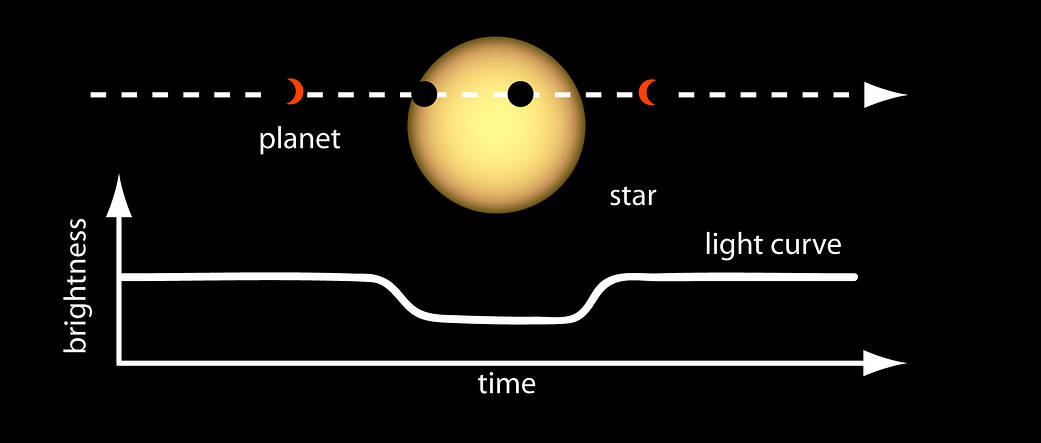
\includegraphics[width=\textwidth]{Transit_Methode.jpg}
	\caption{Transit method}
	\label{fig:mesh2}
\end{figure}


At the current state of the art, there is no way to watch a planet, which orbits a star thausends of lightyears away. To prove its existence, the corresponding star itself is watched over a long period of time and its luminosity is recorded. This data is captured in light curves. A reappearing dent in this light curve can indicate an object which orbits the star and periodically obstructs the line of sight of the telescope/camera. This is clarified in figure \ref{fig:mesh2}. To exclude the possibility of a coincidence, this change in the luminosity of the star has to be detected three times with the same time interval. Other than proving the existence of an exoplanet, more information can be derived from the course of the light curve. It is possible to calculate for example the planets radius, its inclination and its distance to the star. Through spectral analysis, statements about the atmospheric composition, the temperature and the albedo of the planet can be made.           
\newline 
This indirect method is dependent on the planets orbit crossing the line between telescope and star. The chance of this happening is only around 1\%. PLATO will counter this problem by watching thousands of stars at once over years. Statistically it will have discovered ... stars by the end of the mission.  
 
\section{The fine guidance System}
The requirements for the fine guidance system are described here.